\documentclass[project_eva.tex]{subfiles}
\begin{document}

\section*{Interaction}

\subsection*{Emotion recognition}
Eva is able to recognize ``emotions'' in the words spoken by the user, this is done with speech recognition \footnote{See 
Technical Document}. By comparing the recognized words with a list of positively and 
negatively loaded words, Eva is able to distinguish positive and negative feedback. This is the simplest form of emotion 
recognition that works efficiently, given that the speech recognition module works good enough \footnote{Advised by Dr. ir. 
Pascal Wiggers}. 

Another asset for simple emotion recognition would be smile detection, since it is not hard to detect smiles on human faces 
(look for white teeth and lifted mouth corners \footnote{Advised by Dr.Joost Broekens}). An implementation of emotion 
detection already exists \cite{autosmiley}, but this was not used in this project due to time 
constraints and inability to compile the program because of deprecated code.
 
\subsection*{Emotion expression}
blabla 

\subsection*{Eye contact}
Eva is able to detect faces and track them with her head. This makes her look into the eyes of the person who is talking to 
her, which stimulates user interaction. Because people are used to looking into the other's eyes during a conversation, 
this feature provides a familiar and natural way for elderly to communicate with Eva. The face detection is done using the face detection example in OpenCV \footnote{http://opencv.willowgarage.com/wiki/FaceDetection}, which utilizes Haar-like features.

\subsection*{Commands}
To give orders to Eva, one only needs to speak to her in English (Other languages are not yet supported). Eva uses speech 
recognition to listen to the spoken sentences and searches for keywords, which correspond to certain actions. An example 
would be getting juice whenever the word ``juice'' is heard in a sentence. This is done because the current technology for 
speech recognition is too unreliable to detect words accurate, so instead of listening to whole sentences (which are harder 
to recognize), Eva only listens to the important words that matter.

Being able to recognize commands through speech was a necessary feature for Eva because elder people are used to speaking 
with natural language. By using speech recognition, it is not needed for elderly to learn a new way to communicate with 
Eva, which makes it easier for them to accept and to make use of Eva.

\newpage

\section*{Object manipulation}
\subsection*{Object recognition}
For object recognition, the tabletop object detector from ROS is used. This algorithm detects rotational symmetric objects on a table by segmenting clusters above the tabletop, which are compared to known models in a given database. Each cluster is then fitted to each model in the database and when a good fit is found, the position of the found object will be returned so Eva can grab the object. Because the tabletop detector only uses segments to detect objects, it can only recognize objects by form, meaning that two different products with the same form can be seen as the same object. Also, the models are inserted in the database beforehand and have to be created by the user self.

To detect the tabletop, fast plane detection is used \cite{plane}, which 
searches for planes. the biggest recognized plane will be seen as a tabletop, meaning that a wall can also be seen as a 
tabletop if Eva is seeing one.

For more information about the tabletop detector, please refer to \url{http://www.ros.org/wiki/tabletop\_object\_detector} \cite{tabletop}.

The tabletop object detector was used in this project because the results in segmenting and distinguishing the objects were better than the package used previously, namely RoboEarth \cite{Roboearth}. Although it was easier to add objects to the database of RoboEarth, the detection of objects was not reliable, thus making the tabletop object detector the better option. However, since RoboEarth is still a work in progress, it is anticipated that detection in RoboEarth happens with more success in the future, so it will be a good alternative if improvements are made.

\subsection*{Eva's arm}
blabla

\subsection*{Inverse kinematics}
As mentioned in the previous section, Eva's arm uses two motors to position the gripper: one for moving the arm sideways 
and one for moving the arm in height. In order to position the gripper to a desired position, inverse kinematics are used 
to calculate the joint positions of the motors for a given coordinate in the coordinate frame of the arm. On the other 
hand, forward kinematics are used to calculate the current position of the arm, which is used as feedback for positioning 
the gripper. 

Although this is a deprecated way to position the gripper because of the complexity of inverse kinematics  (Nowadays, 
jacobians \cite{jacobian} [p. 65-69] are used to solve the inverse twist 
problem for the gripper which enables positioning by speed control), in Eva's case, this problem was very easy to solve 
because her arm only has two degrees of freedom. 

Given the coordinates x and z, the inverse kinematics of the arm are solved by the following formulas. Note that the y 
coordinate of the gripper depends on the z coordinate because the link in the middle always stays horizontal, so it is not 
necessary to take that into the calculations. The first formula calculates the angle for the shoulder, the second formula 
calculates the angle for the ``wrist''. See also \ref{fig:IK0} , \ref{fig:IK1} and \ref{fig:IK2} for drawings used for the calculations.

\begin{equation*}
\alpha = \arcsin(z_4/L1)
\end{equation*}

\begin{equation*}
\beta = -1 * \arcsin(x_4/(L3 + L4))
\end{equation*}

Also, the following formulas are used to 
keep track of the position of the gripper, given an angle $\alpha$ for the 
shoulder and an angle $\beta$ for the ``wrist'' link:

\begin{equation*}
z = \sin(\alpha)*L1
\end{equation*}

\begin{equation*}
x = \sin(-1 * \beta)*(L3 + L4)
\end{equation*}

\begin{figure}[ht!]
	\centering
	\mbox{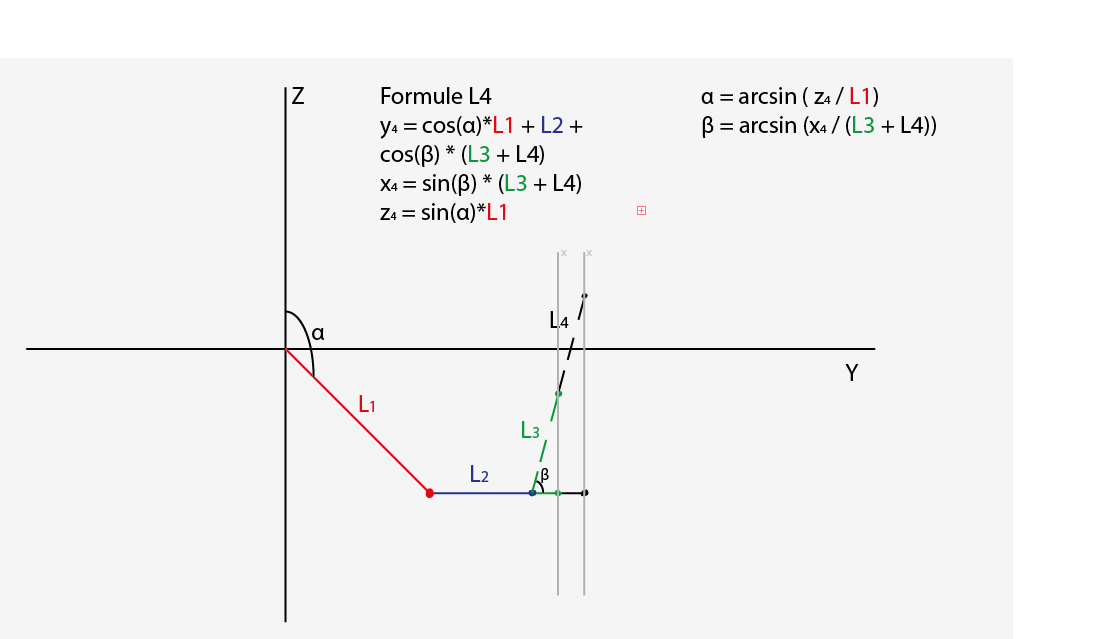
\includegraphics[width=0.5\textwidth]{Images/3d_zijenbovenaanzicht.png}}
	\caption{Side and top view of the arm with calculations of the kinematics}
	\label{fig:IK0}
\end{figure}

\begin{figure}[ht!]
	\centering
	\mbox{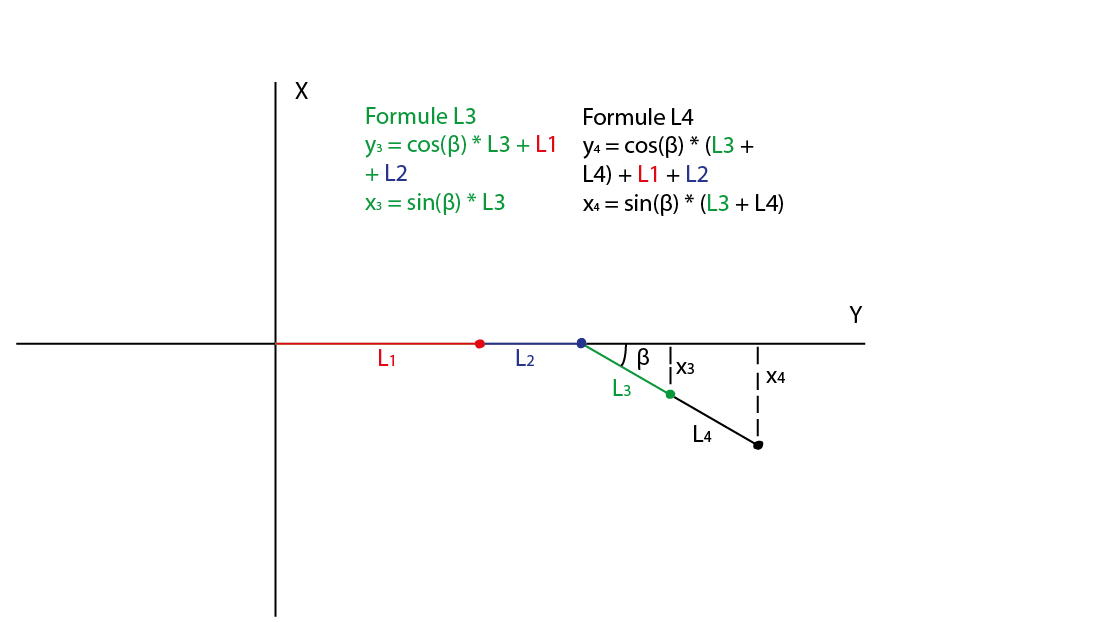
\includegraphics[width=0.5\textwidth]{Images/2d_bovenaanzicht.png}}
	\caption{Top view of the arm with calculations of the kinematics}
	\label{fig:IK1}
\end{figure}

\begin{figure}[ht!]
	\centering
	\mbox{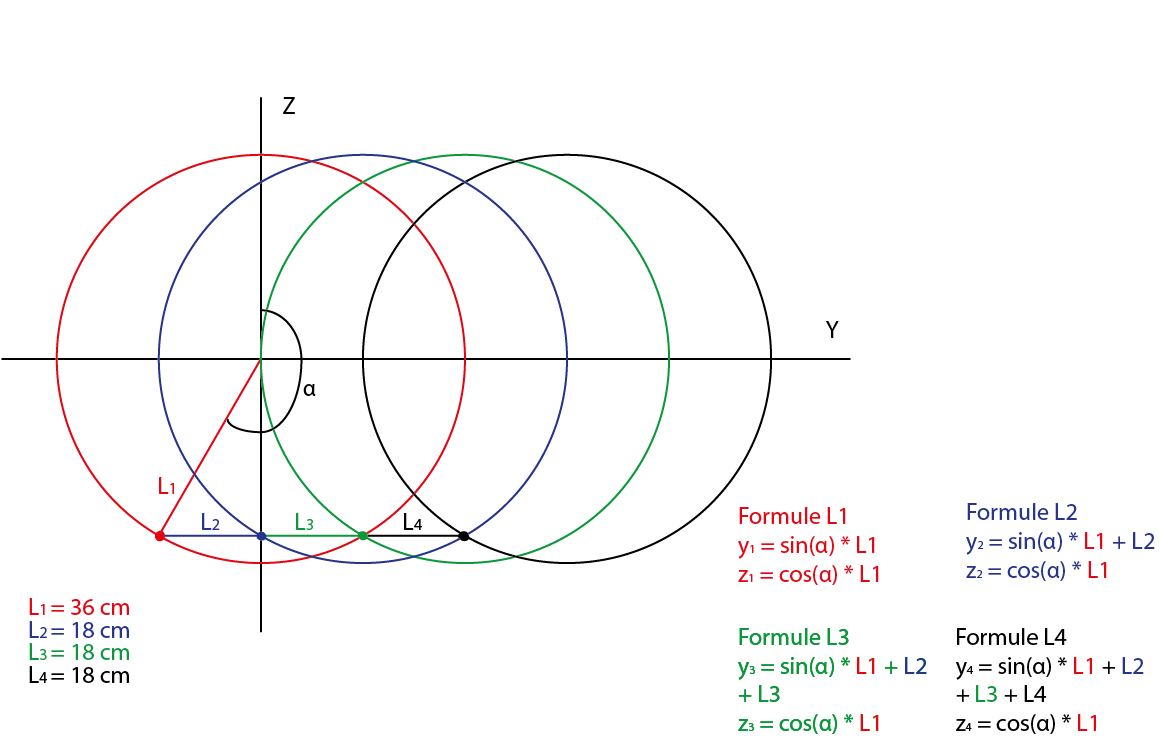
\includegraphics[width=0.5\textwidth]{Images/2d_zijaanzicht.png}}
	\caption{Side view of the arm with calculations of the kinematics}
	\label{fig:IK2}
\end{figure}

\section*{Navigation}
Navigating Eva in an environment exists of three parts. Firstly, Eva needs to know her surroundings; she needs to map out the environment. Secondly, she needs to plan a path from where she is to where she wants to go. Thirdly she needs to know how to execute this path as good as she can.
\subsection*{Map creation}
The GMapping package in ROS was used to create a map of the environment. GMapping\footnote{http://www.openslam.org/gmapping.html} is a SLAM algorithm, which stands for \textit{Simultaneous Localization And Mapping}. The algorithm takes in laserscan and odometry data and this data is converted into a map. There is no laser present on Eva, so this data had to be substituted by Kinect data, which is an easy conversion.

At this stage there is a map created by GMapping, but in .pgm format. Recast\footnote{http://code.google.com/p/recastnavigation/} is used to convert a map into a navigation mesh, which is later used to determine a path from point A to point B, however Recast accepts only maps of the format .obj, a 3D representation format\footnote{http://en.wikipedia.org/wiki/Wavefront\_.obj\_file}. To convert from .pgm to .obj a custom converter had to be written, more information on this can be found in the technical document. Recast is then ready to create a navigation mesh on the map. This mesh defines where Eva is allowed to walk, it does so using a set of parameters, of which the most important one is the radius of Eva. With this Recast can determine the walkable areas in the map. This mesh can later on be used to determine paths for Eva.
\subsection*{Global planner}
Originally the navigation stack in ROS was used as global planner. This navigation stack however proved to be a big black box, if it didn't work it was hard to figure out why. On top of that, it required a lot of processing power. The laptop used in Eva could not handle this navigation quickly enough and was sometimes behind on reality. For these reasons and because of earlier experience with a path planner designed for games (which could be applied here too), it was decided to scratch this navigation stack and create one based on Recast/Detour. The efficiency of this path planner is much better, because most of the calculation is done before navigating and it is optimized to be functional in games with many agents requesting new paths.
\subsubsection*{Planning}
Calculating paths on the generated navigation mesh is done using Detour, which is supplied together with Recast. Detour is handed a starting location (the position of Eva) and a goal location. Using the navigation mesh supplied earlier, a path is calculated (ideally exactly on the goal location, but if this is not on the navigation mesh or unreachable, it gets as close as possible). The path is described by waypoints, where the number of waypoints can be increased, making the path smoother.
\subsubsection*{Executing a path}
Originally Eva would strictly follow this path. What this means is that she would keep rotating until she was facing the path, then drive forward until she reached a waypoint and then rotate again until she faced the next waypoint. This looked very unnatural and very static. 

For this reason a new way to execute the path was designed. This enabled Eva to deviate from the path just slightly, enough to take corners while still driving forward. The idea behind this new way of executing the path, is that Eva looks a certain distance forward on the path and tries to drive to that point. When Eva is nearing a corner, her focus point is just a bit beyond this corner, thus she cuts it slightly while still driving forward. To prevent her from flying out of a corner, the forward speed is reduced as the angular speed increases. In effect this means that when she is taking corners, she slows down and after having taken the corner speeds up again. This path execution can be seen in figure \ref{fig:global_path}. The green line is the complete path, whereas the black line points towards the focus point of Eva. The longer this line, the faster she drives forward. In simple words this black line can be seen as a spring attached to Eva.
\begin{figure}[ht!]
	\centering
	\mbox{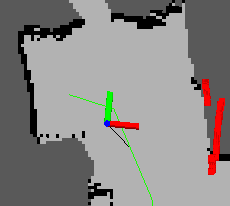
\includegraphics[scale=0.4]{Images/global_path.png}}
	\caption{Eva executes a (global) path.}
	\label{fig:global_path}
\end{figure}

\subsection*{Object avoidance}
Object avoidance is needed for Eva to keep herself safe, but also to keep the environment safe for her. Eva uses ultrasone 
sensors to listen to the objects in her environment and scales the speeds of her wheels according to the distance to the 
detected object and the position of this object. Eva has six sensors in front, two in the back and one on each side. The sensors in the front are used in units (see figure). So if Eva hears an object on the left, she will go right and vice versa. In essence, Eva avoids objects as a Braitenberg vehicle 
\cite{braitenberg} [p. 8]. For more information about object avoidance, see the 
technical document.

\end{document}